% Needs 2 passes, as the overlay is used!
\documentclass[margin=2pt]{standalone}
\usepackage[table]{xcolor}
\usepackage[utf8]{inputenc}
\usepackage[T1]{fontenc}

\usepackage{tikz}
\usepackage{helvet}
\usepackage{amsmath}
\usepackage{array}
\usepackage{tabularray}
\usepackage{etoolbox}

\renewcommand\familydefault\sfdefault

\newcommand{\lMode}{Mode}
\newcommand{\lOwner}{Owner}
\newcommand{\lGroup}{Group}
\newcommand{\lTimestamps}{Timestamps (3)}
\newcommand{\lSize}{Size}
\newcommand{\lBlockCount}{Block count}
\newcommand{\lBlockDirect}{Direct blocks}
\newcommand{\lBlockIndirectSingle}{Single indirect}
\newcommand{\lBlockIndirectDouble}{Double indirect}
\newcommand{\lBlockIndirectTriple}{Triple indirect}
\newcommand{\lBlockIndirectFirst}{direct\\[-.4em]\vdots}
\newcommand{\lBlockIndirectSecond}{single\\\vdots\\indir.}
\newcommand{\lBlockIndirectThird}{double\\[-.4em]\vdots\\indir.}

\newtoggle{czech}
\settoggle{czech}{true}
\iftoggle{czech} {
    \renewcommand{\lMode}{Mód}
    \renewcommand{\lOwner}{Vlastník}
    \renewcommand{\lGroup}{Skupina}
    \renewcommand{\lTimestamps}{Časová razítka (3)}
    \renewcommand{\lSize}{Velikost}
    \renewcommand{\lBlockCount}{Čítač linků}
    \renewcommand{\lBlockDirect}{Přímé linky}
    \renewcommand{\lBlockIndirectSingle}{Nepřímé jednoduché}
    \renewcommand{\lBlockIndirectDouble}{Nepřímé dvoucesté}
    \renewcommand{\lBlockIndirectTriple}{Nepřímé trojcesté}
    \renewcommand{\lBlockIndirectFirst}{přímá\\[-.4em]\vdots}
    \renewcommand{\lBlockIndirectSecond}{nepř.\\[-.4em]\vdots\\jedn.}
    \renewcommand{\lBlockIndirectThird}{nepř.\\[-.4em]\vdots\\dvou.}
}

\usetikzlibrary{intersections, shapes.arrows, spath3, shapes.geometric, fit, backgrounds, calc, tikzmark, matrix}
\usetikzlibrary{shapes.multipart} 

\definecolor{themeBlue}{RGB}{1, 103, 143}
\definecolor{themeOrange}{RGB}{221, 109, 16}
\definecolor{themeTeal}{RGB}{18, 54, 69}
\definecolor{themeGrey}{RGB}{120, 121, 124}
\definecolor{themeGreen}{RGB}{193, 225, 193}



\begin{document}
    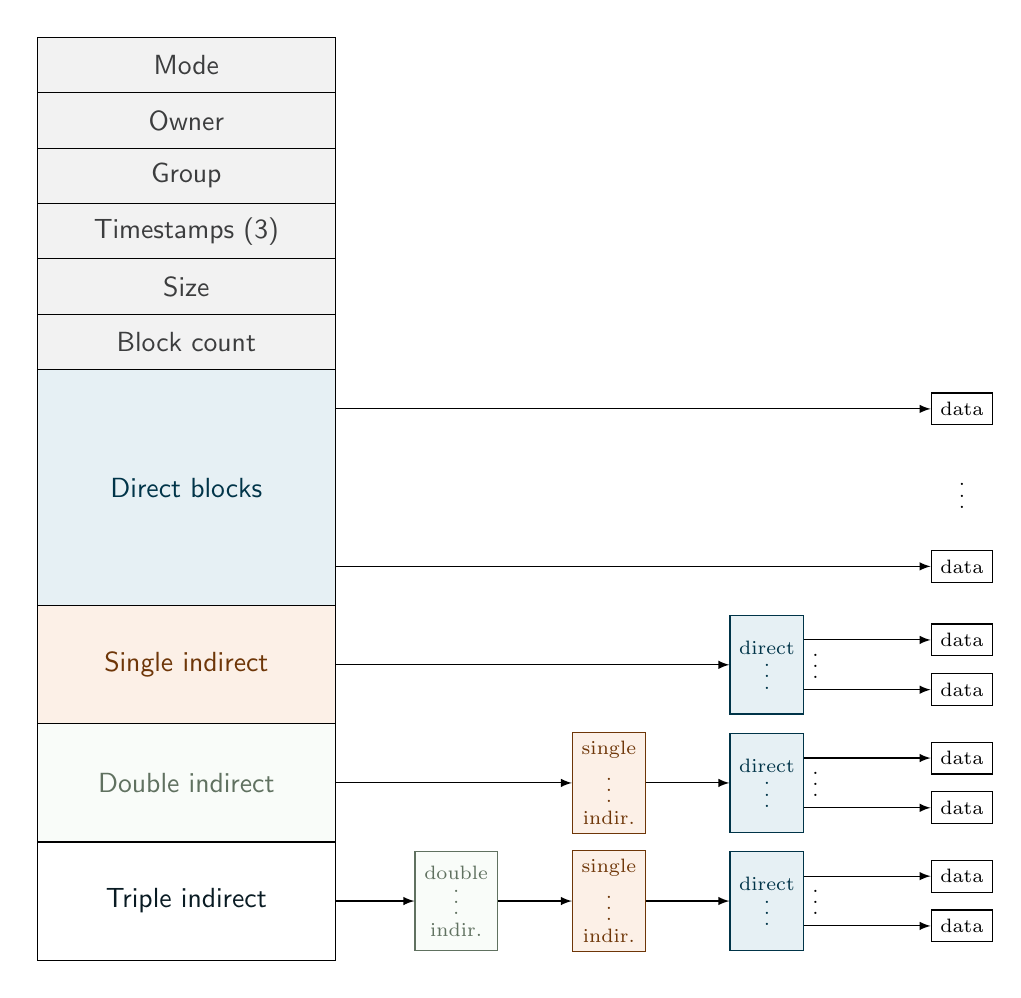
\begin{tikzpicture} [
        font=\sffamily,
        head color/.style args={#1/#2}{
        row 1 column #1/.append style={nodes={fill=#2}}},
        % swap order of row and column styles
        matrix/inner style order={
            every cell,
            row, even odd row,
            column, even odd column,
            cell 
        },
        c/.style={align=center}
    ]

\matrix [
   matrix of nodes, nodes in empty cells,
   row sep=-\pgflinewidth, column sep=-\pgflinewidth,
   nodes={c, draw, text width=3.5cm, align=center,
          minimum height=2em, anchor=center, inner sep=4pt},
   row 1/.style= {nodes={fill=themeGrey!10}},
   row 2/.style= {nodes={fill=themeGrey!10}},
   row 3/.style= {nodes={fill=themeGrey!10}},
   row 4/.style= {nodes={fill=themeGrey!10}},
   row 5/.style= {nodes={fill=themeGrey!10}},
   row 6/.style= {nodes={fill=themeGrey!10}},
   row 7/.style= {nodes={fill=themeBlue!10, minimum height=3cm}},
   row 8/.style= {nodes={fill=themeOrange!10, minimum height=1.5cm}},
   row 9/.style= {nodes={fill=themeGreen!10, minimum height=1.5cm}},
   row 10/.style= {nodes={minimum height=1.5cm}},
  ] (m)
  {
    \textcolor{themeGrey!50!black}{\lMode} \\
    \textcolor{themeGrey!50!black}{\lOwner} \\
    \textcolor{themeGrey!50!black}{\lGroup} \\
    \textcolor{themeGrey!50!black}{\lTimestamps} \\
    \textcolor{themeGrey!50!black}{\lSize} \\
    \textcolor{themeGrey!50!black}{\lBlockCount} \\
    \textcolor{themeBlue!50!black}{\lBlockDirect} \\
    \textcolor{themeOrange!50!black}{\lBlockIndirectSingle} \\
    \textcolor{themeGreen!50!black}{\lBlockIndirectDouble} \\
    \textcolor{themeTeal!50!black}{\lBlockIndirectTriple} \\
  };

    \draw (m-10-1.east) 
        ++ (1,0) node[draw, themeGreen!50!black, fill=themeGreen!10, font=\scriptsize, minimum width=0.9cm, minimum height=1.25cm, align=center, anchor=west] (indir-3 3) {\lBlockIndirectThird}
        ++ (2,0) node[draw, themeOrange!50!black, fill=themeOrange!10, font=\scriptsize, minimum width=0.9cm, minimum height=1.25cm, align=center, anchor=west] (indir-3 2) {\lBlockIndirectSecond} 
        ++ (2,0) node[draw, themeBlue!50!black, fill=themeBlue!10,
        font=\scriptsize, minimum width=0.9cm, minimum height=1.25cm, align=center, anchor=west] (indir-3 1) {\lBlockIndirectFirst};

    \draw (indir-3 2|-m-9-1.east) node[draw, themeOrange!50!black, fill=themeOrange!10, font=\scriptsize, minimum width=0.9cm, minimum height=1.25cm, align=center] (indir-2 2) {\lBlockIndirectSecond};

    \draw (indir-3 1|-m-9-1.east) node[draw, themeBlue!50!black, fill=themeBlue!10, font=\scriptsize, minimum width=0.9cm, minimum height=1.25cm, align=center] (indir-2 1) {\lBlockIndirectFirst};

    \draw (indir-3 1|-m-8-1.east) node[draw, themeBlue!50!black, fill=themeBlue!10, font=\scriptsize, minimum width=0.9cm, minimum height=1.25cm, align=center] (indir-1 1) {\lBlockIndirectFirst};

    \draw[-latex] (m-8-1.east) -- (indir-1 1);
    \draw[-latex] (m-9-1.east) -- (indir-2 2);
    \draw[-latex] (m-10-1.east) -- (indir-3 3);

    \draw[-latex] (indir-2 2) -- (indir-2 1);
    \draw[-latex] (indir-3 2) -- (indir-3 1);
    
    \draw[-latex] (indir-3 3) -- (indir-3 2);

    \foreach \i in {3, ..., 1} {
        \draw ($ (indir-\i\space1.north east)!.25!(indir-\i\space1.south east) $) coordinate (indir-\i\space edge 1) ++(2, 0) node[draw, font=\scriptsize] (indir-\i\space data 1) {data};
        \draw ($ (indir-\i\space1.north east)!.75!(indir-\i\space1.south east) $) coordinate (indir-\i\space edge 0)   ++(2, 0) node[draw, font=\scriptsize] (indir-\i\space data 0) {data};
    
        \draw[-latex] (indir-\i\space edge 0) -- (indir-\i\space data 0);
        \draw[-latex] (indir-\i\space edge 1) -- (indir-\i\space data 1);
        
        \draw ($ (indir-\i\space edge 1.east)!.5!(indir-\i\space edge 0.east) +(.1, 0) $) node[anchor=center, right, font=\scriptsize, inner sep=0, outer sep=0, yshift=2.5pt] {\vdots};
    }

    \draw (indir-1 data 1|-m-7-1) ++(0, 1) node[draw, font=\scriptsize] (dir data 2) {data};
    \draw (indir-1 data 1|-m-7-1) node[font=\scriptsize] (dir data 1) {\vdots};
    \draw (indir-1 data 1|-m-7-1) ++(0, -1) node[draw, font=\scriptsize] (dir data 0) {data};

    \draw[-latex] (m-7-1.east|-dir data 0) -- (dir data 0);
    \draw[-latex] (m-7-1.east|-dir data 2) -- (dir data 2);

    \end{tikzpicture}
\end{document}